\documentclass[output=paper]{langscibook}
\ChapterDOI{10.5281/zenodo.6762282}

\author{Rosa {Vallejos Yopán}\affiliation{University of New Mexico} and Fernando García Rivera\affiliation{FORMABIAP} and Haydée Rosales Alvarado\affiliation{FORMABIAP}}
\title{Indigenous languages in higher education: Case studies from the Amazon of Peru}
\abstract{This study examines the role of two indigenous languages in higher education in the Amazon of Peru. It looks at efforts to implement Kukama and Kichwa as key components in the teacher training model developed by the Programa de Formación de Maestros Bilingües de la Amazonía Peruana (henceforth FORMABIAP for its initials in Spanish). At present, Kukama and Kichwa are at different points of UNESCO’s endangerment scale. Teaching them in higher education is part of a more comprehensive commitment to build culturally and linguistically appropriate education for Amazonian indigenous groups. This chapter documents several components of the FORMABIAP project. We look at a sample of eight FORMABIAP’s alumni, five Kukamas and three Kichwas, to investigate and reflect on the overall outcomes of their learning process. In addition, we survey the profiles of the instructors, the structure of the language classes, and their communities of practice. An important finding of this study is that endangered languages can be relearned by heritage speakers in a combination of naturalistic and well-structured instructional settings. We conclude that the assessment of these relearning processes needs to be holistic, going far beyond linguistic proficiency. In the Amazonian context, at the center of it all are language attitudes, sense of cultural membership, and the learners’ positioning with respect to the aspirations of their communities and indigenous organizations. Although the general teaching components can be in fact planned for several ethnic groups, the implementation of the proposals and the evaluation of the outcomes must be done individually and by the indigenous group to capture the uniqueness of each sociolinguistic context.
\keywords{indigenous language, heritage language, Peruvian Amazonia, Kukama, Kichwa}
}

\IfFileExists{../localcommands.tex}{%hack to check whether this is being compiled as part of a collection or standalone
  \addbibresource{../localbibliography.bib}
  % add all extra packages you need to load to this file

\usepackage{tabularx,multicol}
\usepackage{url}
\usepackage{soul}
\usepackage{longtable, xltabular}
\urlstyle{same}

\usepackage{listings}
\lstset{basicstyle=\ttfamily,tabsize=2,breaklines=true}

\usepackage{langsci-basic}
\usepackage{langsci-optional}
\usepackage{langsci-lgr}

\usepackage{todonotes}

\usepackage{makecell}

\usepackage{enumitem}
\usepackage{multirow}
\usepackage{langsci-branding}
\usepackage{langsci-gb4e}

  \newcommand*{\orcid}{}

\newcommand{\togglepaper}[1][0]{
%   \bibliography{../localbibliography}
    \papernote{\scriptsize\normalfont
    \theauthor.
    \titleTemp.
    To appear in:
    Change Volume Editor \& in localcommands.tex
    Change volume title in localcommands.tex
    Berlin: Language Science Press. [preliminary page numbering]
  }
  \pagenumbering{roman}
  \setcounter{chapter}{#1}
  \addtocounter{chapter}{-1}
}

% \newcommand{\keywords}[1]{\par\textbf{Keywords: #1}}

\renewcommand{\lsChapterFooterSize}{\footnotesize}

  %% hyphenation points for line breaks
%% Normally, automatic hyphenation in LaTeX is very good
%% If a word is mis-hyphenated, add it to this file
%%
%% add information to TeX file before \begin{document} with:
%% %% hyphenation points for line breaks
%% Normally, automatic hyphenation in LaTeX is very good
%% If a word is mis-hyphenated, add it to this file
%%
%% add information to TeX file before \begin{document} with:
%% %% hyphenation points for line breaks
%% Normally, automatic hyphenation in LaTeX is very good
%% If a word is mis-hyphenated, add it to this file
%%
%% add information to TeX file before \begin{document} with:
%% \include{localhyphenation}
\hyphenation{
anaph-o-ra
Dor-drecht
Ku-ka-ma
pre-dom-i-nant-ly
prog-ress
teach-er
Ri-ve-ra
}

\hyphenation{
anaph-o-ra
Dor-drecht
Ku-ka-ma
pre-dom-i-nant-ly
prog-ress
teach-er
Ri-ve-ra
}

\hyphenation{
anaph-o-ra
Dor-drecht
Ku-ka-ma
pre-dom-i-nant-ly
prog-ress
teach-er
Ri-ve-ra
}

  %\togglepaper[]
}{}

\shorttitlerunninghead{Indigenous languages in higher education: Case studies from the Amazon}
\begin{document}
\maketitle

\section{Introduction}\label{sec:7:1}
The present study deals with relearning processes of endangered Amazonian languages in the context of FORMABIAP (more details at \href{http://www.formabiap.org}{{www.formabiap.org}}). The Amazon Basin is characterized as one of the most culturally and linguistically diverse areas in the world, with about 300 languages belonging to twenty or so language families, plus dozens of genetic isolates \citep{Queixalós2009}. Nevertheless, Amazonian languages are, for the most part, both poorly documented and highly endangered. The majority of these languages are spoken by relatively small speech communities, compared to Spanish or Portuguese, the two major languages with which they coexist in highly asymmetrical relationships.

\begin{sloppypar}
This chapter focuses on two Amazonian languages: Kukama-Kukamiria (henceforth Kukama) and Kichwa. Their territories are located in the \textit{Loreto} region of Peru. Loreto hosts an extreme linguistic diversity, which includes about 23 languages (\citealt{SolísFonseca2009}; \citealt{Queixalós2009}). However, the speakers of these languages represent only a small percentage of the total population in the region. According to census data from Peru’s \textit{Instituto Nacional de Estadística e Informática} \citep{INEI2017}, 9.8\% of the population in Loreto self-identify as a member of an indigenous group, yet only 6.4\% of them declare to have learned to speak in an indigenous language. These statistics illustrate the increasing social pressure to learn, and ultimately shift to, Spanish.
\end{sloppypar}

\begin{sloppypar}
Languages such as Kukama and Kichwa continue to lose ground in daily use. By including indigenous languages as part of a teaching training program, FORMABIAP aims to counter the progression of rampant language loss. However, data regarding the outcomes of relearning these ancestral languages by heritage speakers do not exist. This is particularly important given that these speakers are, or will eventually be, in charge of teaching these languages in their communities. It is often mentioned that due to their limited command in the ancestral languages, heritage speakers lack the ability to teach these languages (cf. \citealt{LópezGarcía2016}: 127). However, no study has ever attempted to explore how much heritage speakers have actually achieved in the process of relearning their languages. Importantly, in the context explored here, this process does not end at their graduation from FORMABIAP, but continues as they teach the languages to children and engage with other speakers in the linguistic and cultural reanimation of their communities.
\end{sloppypar}

This document aims to start a conversation regarding both heritage language teaching and assessment in the Amazonian context. We look at original empirical data collected from eight heritage speakers and offer the first attempt to understand this relearning process in higher education. An additional aim of the paper is to identify patterns of use, as well as areas of improvement, in the speech of heritage speakers in order to contribute to curricula development. An important finding of this study is that all the participants exhibit various degrees of language expertise. Thus, indigenous heritage languages can be relearned in a combination of naturalistic and well-structured instructional settings, as the outcomes of the multifaceted approach implemented by FORMABIAP are both tangible and substantial.

\section{Local context}\label{sec:7:2}

Any formulation of pedagogical proposals requires a prior characterization of the sociocultural and linguistic contexts of the communities and of the students themselves. In this section, we set the background for the study.

\subsection{Kukama}

The Kukamas live in small villages spread along several Amazonian rivers. According to the parameters provided by UNESCO \citep{Moseley2010}, the Kukama language is severely to critically endangered. The total number of Kukamas is estimated at 20,000. However, the \citealt{INEI2017} census indicates that only 1,185 individuals have learned to speak this ancestral language, and 82.6\% of them live in the Loreto region.\footnote{{According to \citep{INEI2017}, 9.7\% of the 1185 Kukamas live in Lima/Callao, 3.8\% in Ucayali, and the remaining 4\% are spread throughout the country.}} Most of the remaining fluent speakers are elders, and certainly none of them are monolingual in Kukama \citep{Vallejos2016b}. Children are no longer learning the language, as natural processes of language transmission have been interrupted more than five decades ago. Over the years, a growing concern with respect to the vitality of the language has become evident within the speech community itself, which has resulted in a number of revitalization initiatives. These efforts are being implemented mainly through formal education. As a result, it is possible to find different types of speakers of Kukama, in the sense of \citet{GrinevaldBert2011}, including traditional speakers, latent speakers, neo-speakers, and rememberers \citep{Vallejos2016b}.

One of Kukama’s most salient typological features is a morphological distinction between male and female speech in several grammatical categories. Major grammatical categories like person, number, tense, and modality are conveyed by positionally-fixed clitics. Five tense clitics encode three degrees of distance into the past and two into the future. There is a four-way epistemic modal system encoding via second position clitics. In Kukama there is neither case marking nor affixal indexation of core participants to express grammatical relations. In main clauses, SVO is the pragmatically unmarked constituent order. While OSV is employed with salient objects, SOV is only possible if the verb is marked by progressive aspect. Oblique phrases are marked by postposition, and clauses are linked by dedicated adverbial subordinators. Clause nominalization is a central subordination strategy, particularly in relativization.

\subsection{Kichwa}\label{sec:7:2.2}

The Kichwas live in the basins of the Napo, Putumayo, Pastaza and Tigre rivers, in the Loreto region in Peru. Those who live in the basins of the Napo and Putumayo rivers call themselves \textit{Napu Runas} and those who live in the Pastaza and Tigre rivers call themselves \textit{Ingas}. They are also located in the San Martín region, known as \textit{Lamistas}, and in Madre de Dios region, known as \textit{Santarrosinos}. According to the last census, 99\% of the Kichwa live in Loreto, and only 1\% live in other regions. The Kichwa speakers who live along the Napo River are the descendants of Ecuadorian Kichwa populations called \textit{Quijos} (\citealt{MayorBodmer2009}). The Kichwa themselves assert that their parents or grandparents came from Ecuador, and a group of them migrated from the Napo River to Madre de Dios during the time of rubber extraction. Although the Ministry of Education of Peru mentions that Kichwa is a variety of the Quechua language, in the last national census \citep{INEI2017}, Kichwa is listed as a different language than Quechua. According to this census, 5,751 declared that Kichwa is the language in which they learned to speak. Although the number of Kichwa speakers in Peru seems to be very small, their linguistic kinship with the Quechua-speaking population (3,799,780 according to \citealt{INEI2017}) relativizes this situation. Kichwa exists in a range of sociolinguistic situations, from communities where this language is the main means of communication among all generations, to communities where Spanish has almost completely replaced Kichwa (see \sectref{sec:7:2.4}).

The Kichwa varieties are part of the Quechua linguistic family. There are, however, important cultural and linguistic differences between Kichwa and Quechua. From a cultural perspective, due to their geographical location in the Peruvian Amazon, the Kichwas’ worldview is closer to other Amazonian peoples, including the conception of territory as a fundamental element of life. Perhaps the most salient phonological difference between Kichwa and Quechua is that Quechua makes a distinction between post velar /q/ and velar /k/, Kichwa does not make this distinction. Regarding its typological profile, Kichwa is characterized as an agglutinating language with suffixal morphology. The preferential order of constituents is SOV, although SVO, OVS are also possible. Grammatical relations are encoded through case marking and verb indexation. Finite verbs take TAM suffixes. Adnominal possession is expresses via a genitive marker suffixed to the possessor.

\subsection{Speaker types in endangered language contexts}

Amazonian languages exhibit different degrees of endangerment. Speech communities of endangered languages typically comprise several types of speakers who show variance in competence. \citet{GrinevaldBert2011}, building on \citet{Dorian1980}, propose four clusters of variables to identify types of speakers: (i) language competence cluster (level of acquisition attained and degree of individual loss), (ii) sociolinguistic cluster (vitality of language at time of acquisition and the age of the speaker at the time of exposure to the language), (iii) performance cluster (level of use of the language and the attitudes towards the language), (iv) self-evaluation of language skills (which can range from under-evaluation, insecurity and self-denial to over evaluation). The implementation of these four parameters gives the following types of speakers (\tabref{tab:7:1}).

\begin{table}[t]
\caption{Typology of speakers of endangered languages \citep[147]{Vallejos2016b}}
\label{tab:7:1}

\begin{tabularx}{\textwidth}{lQ}
\lsptoprule
Fluent speakers & Also called traditional speakers, they have acquired the language fully and are able to engage in spontaneous conversations. Such speakers are able to provide narratives with very minimal use of borrowings.\\
\tablevspace
Latent-speakers & They demonstrate receptive skills but with varying degrees of production. They have not had regular conversation partners and display modified patterns that can be considered mistakes by fluent speakers.\\
\tablevspace
Rememberers & This category includes speakers with advanced level of attrition often due to traumatic circumstances. They have passive knowledge and very limited productive skills, which usually includes frozen expressions. They may have regained or reacquired some partial use and could be at first inhibited to get involved in revitalization efforts.\\
\tablevspace
Former speakers & They are also called ghost speakers, those who deny any knowledge of the language. This denial is a consequence of strong negative attitudes associated with speaking a language that is usually overpowered by a national language.\\
\tablevspace
Last speaker & This may be a socio-political category; that is, public and social role assigned by a community, or self-attributed. \\
\tablevspace
Neo-speakers & They are the product of revitalization initiatives. They have positive attitudes towards the language and make conscious efforts to learn it. They can achieve a range of proficiency levels and show signs of language obsolescence. \\
\lspbottomrule
\end{tabularx}
\end{table}

FORMABIAP trains neo-speakers, who, if we highlight their cultural ties to the Kukama and Kichwa ethnic groups, are considered \textit{heritage speakers}. These students enter the program with very limited knowledge of their ancestral languages (more details in \sectref{sec:7:5} and \sectref{sec:7:6}).

\subsection{Sociolinguistic contexts}\label{sec:7:2.4}

Concurrent with different speaker types, Amazonian languages are spoken in a variety of sociolinguistic contexts. Considering the social dynamics and the actual use of the indigenous languages and Spanish, it is possible to identify a wide range of complex scenarios. For example, if we take the Kichwa villages along the Napo River in Peru as a reference point, we can identify a continuum in terms of the vitality of the Kichwa language. In the High Napo River (\textit{Alto Napo}), an area close to the Peru-Ecuador border, there are villages such as Chingana and Humandi where children are learning Kichwa as a first language. In those villages, Kichwa is still the dominant language among all the generations, and very few know any Spanish.

In the High Napo region, but further south from the Peru-Ecuador border, there are villages such as Angoteros and Campo Serio where bilingualism in Spanish and Kichwa is gaining ground among male adults. In those villages, Spanish is used in rather limited contexts; note that by the time children start schooling around the age of five, they are predominantly monolinguals in Kichwa. Even further south in the High Napo region, there are villages, such as Ingano Llacta, where bilingualism in Kichwa and Spanish has been extended to the entire population. In these villages, every generation is bilingual. As a result, children are currently learning both languages from birth.

In the Mid Napo River (\textit{Medio Napo}), in villages like Copal Urcu, San Carlos, Rumitumi, Diamante Azul, and San Jorge, the majority of the children and the youth already speak Spanish as a first, and mostly only, language. However, these generations are still exposed to Kichwa during their interactions with their parents and grandparents. The generations of adults and elders communicate among themselves in Kichwa, but they tend to address their children in Spanish. As a result, most of the children and the youth can understand Kichwa, but show very limited production in this language.

In the villages located along the Low Napo River (\textit{Bajo Napo}), the situation is more pressing. In villages such as Lagartococha, Puca Barranca, and San Juan de Yanayacu, Kichwa has been displaced almost completely. Although it is still spoken by elders, and they may use it in sporadic situations among themselves, Spanish is already the only language of daily communication for all generations. Beyond the Napo River, the Kichwa villages located along the Pastaza River and the Tigre River also show displacement of Kichwa in favor of Spanish, mainly among children and the younger generation.

As for the Kukama villages, most of them have experienced language shift in favor of Spanish, similar to the last scenario discussed for Kichwa. Nowadays, Kukama is only known by elders, and they use it in very restricted contexts. However, there seems to be a difference between the Kukamas and the Kichwas. The Kukamas are more aware of the loss of their language, and in the last decade they have started to express their concerns more openly. In some regions, there are ongoing movements of cultural re-appropriation to reconnect with their roots, and relearning their heritage language is part of this movement.

Note that the possibilities for re-learning the indigenous language decreases from one scenario to another. Taking Kichwa, again, as a reference, it is possible to say that natural language transmission is almost guaranteed in the first scenario. The second and third scenarios result in different degrees of bilingualism; these new language practices tend to go hand in hand with negative attitudes towards the indigenous language. In cases like this, children learning the indigenous language as a first language is no longer guaranteed. In the fourth scenario, children are not acquiring the indigenous language as a first language, but the context is favorable for re\nobreakdash-learning it with heritage language methodologies. In the fifth scenario, the functionality of the indigenous language is extremely limited, and so is the possibility of learning the indigenous language without a well-thought-out revitalization effort.

Notably, one of the many challenges FORMABIAP faces to teach indigenous languages is that its students come from all these different scenarios.

\section{The FORMABIAP Program}\label{sec:7:3}

FORMABIAP began its activities in 1988, as a result of an agreement between the Ministry of Education of Peru, the \textit{Corporación Departamental de Desarrollo de Loreto} (CORDELOR), the \textit{Asociación Interétnica de la Selva Peruana} (AIDESEP), and the Italian NGO Terra Nuova. FORMABIAP was created as a program to train indigenous teachers in intercultural bilingual education (IBE) within the framework of a Pedagogical Higher Education Institute, based in the city of Iquitos. From its inception, FORMABIAP was a pioneer model for a genuine collaboration between the government and a national indigenous organization. The role of indigenous specialists and scholars in the teacher training process, as well as the participation of community members in the development of the curricula for elementary education are some of the key components of its success. In its 32 years of work, FORMABIAP has trained 1,213 indigenous teachers from 16 Amazonian ethnic groups, who have taught an estimated 363,900 Amazonian children \citep{TrapnellEtAl2018}.

FORMABIAP considers that languages and education must be approached from the specific social contexts in which the project operates, and from a political and historical vision that allows its students to understand how the processes of colonial domination have influenced the current situation of the indigenous languages \citep[38]{TrapnellEtAl2018}. At the beginning of the FORMABIAP project, most students had an indigenous language as their L1, with the exception of the Kukamas who were mostly monolingual in Spanish. Over the years, the sociolinguistic landscape has become more heterogeneous and complex to address. On the one hand, there is now a greater number of students with serious limitations in oral Spanish. On the other hand, the number of students that have Spanish as a first language has increased.

\subsection{Why heritage language instruction in FORMABIAP}

A second language is any language an individual learns in addition to their first language, and no previous knowledge of this language is implied. In contrast, a heritage language entails certain exposure to the target language during childhood, as well as a cultural connection to the language through family, ancestors, community, or country of origin. In this view, a heritage language can be an indigenous language that underwent displacement (i.e. Kukama and Kichwa in Peru) or an immigrant language (i.e. Spanish in the United States or Turkish in Germany). In a narrow definition, heritage learners are bilinguals, but the language they learned in childhood at home is no longer their dominant language; instead, they are dominant in the hegemonic language of the society in which they live. In a broad definition, heritage learners have had at least some input during childhood but did not grow up with this language as a means of communication (\citealt{PolinskyKagan2007}; \citealt{Rothman2009}). As a result, heritage language learners can display widely diverse levels of proficiency (\citealt{Valdés1989,Valdés2005}). In the cases discussed in this article, we adopt a broad definition of heritage learners.

Heritage languages, as all languages, are surrounded by ideologies, from issues of identity and group membership, to views of language as a commodity that question the value of an ancestral language in current times. Other common ideologies relate to who are the “true owners” of a given language, who should have the ultimate say on how the “real language” should sound like, and diverse perceptions regarding language variation and change (see, for instance,  \citealt{LopezOdango2015}). Thus, in multilingual settings such as the Amazon, the development of intercultural communication competence needs to be stressed. This development involves self-reflection concerning language and culture, and it involves attitudinal changes toward one’s own and others’ cultures and languages.

The fact that heritage learners bring some linguistic knowledge from childhood has opened important avenues in second language acquisition research, particularly on the role of age, input, and implicit versus explicit knowledge \citep{Valdés2005}. For example, heritage speakers seem to have an advantage over L2 learners not only with regards to phonology, but also in some aspects of morphology and syntax \citep{Montrul2008}. Issues related to linguistic mechanisms and the types of patterns that emerge in language loss and revitalization contexts \citep{Hinton2001} are also important theoretical questions for language change. The impact of the results of these new lines of research in teaching methodologies continues to be explored (\citealt{Parodi2008}, \citealt{Potowski2018}).

Motivation is critical to language learning, but particularly so in heritage language learning. If cultural heritage is a motivating factor to learn a language, it can promote learner autonomy to continue the learning process beyond the formal settings. This is critical in endangered language contexts where the target language is no longer used in daily communication. For example, leaners of Kukama and Kichwa have to make an effort to build a community of practice in their villages.

Heritage learners can also vary with respect to forms of exposure and age of acquisition (naturalistic process during childhood, formal instructional settings as adults, revitalization contexts guided by elders and activists, etc.), communities of practice, and amount of access to input in the target language. The heritage speakers of Kichwa and Kukama who participated in this study were exposed to their ancestral languages to various degrees during childhood; however, all of the participants manifest a strong cultural connection and a sense of membership to their respective ethnic groups.

\subsection{Profile of learners}\label{sec:7:3.2}

Three decades ago, aspiring Intercultural Bilingual Education (IBE) teachers were older than the average high school graduates in Peru, and many had not completed a secondary education. Most of the students at the time predominantly spoke an indigenous language as their first language, with the exception of the Kukamas. In more recent years, however, the completion of a high school education became a prerequisite to enter \textsc{FORMABIAP}. By going through the complete educational system (i.e. kindergarten, primary, and secondary), in many cases outside their villages, these students have acquired greater proficiency in Spanish than those that entered FORMABIAP 30 years ago. Nevertheless, an unintended consequence is that these new generations have had fewer opportunities to learn the cultural knowledge of their people and their respective indigenous language. As a result, the most recent cohorts of students who come to FORMABIAP show less command of their indigenous languages. That is, the linguistic profile that used to be associated with the Kukamas has now been extended to other indigenous groups, such as the Awajun, Shawi and Kichwa. Note, though, that the Kukamas and Kichwas come with a very limited command of their heritage languages not only ​​because of the formal schooling, but also because the generation of grandparents who speak those languages is declining rapidly.

Under these conditions, the relearning of an indigenous language by the future teachers is even more challenging. But even for students who have an indigenous language as their L1, having had less exposure to that language in the community life entails that it needs to be taught and expanded at the oral and written levels. In several cases, the indigenous language was generally used only in primary education (K-5), and then its use was interrupted at the secondary level. In the Amazon of Peru, secondary education is developed almost exclusively in Spanish. It is then imperative that the new cohorts that join FORMABIAP strengthen their competence in their indigenous languages, as well as their cultural traditions.

However, the demand for learning the indigenous languages arises not only because of FORMABIAP’s institutional mission, but because there are now national IBE policies that demand communicative competence of the indigenous languages in the schools that provide an intercultural bilingual education (\citealt{MinisteriodeEducacióndelPerú2016}). In addition, according to the new official policies, teachers working in communities with heritage indigenous languages must implement cultural and linguistic revitalization \citep{MinistryofEducationofPeru2016}. In those communities, children have access to very few opportunities to listen to the indigenous language because it is spoken only by older people in very restricted contexts. Thus, given that teachers have to teach these heritage languages to the children of these schools, the indigenous language must be relearned as part of their teacher training in FORMABIAP.

\subsection{Profile of instructors}\label{sec:7:3.3}

FORMABIAP hires language and culture \textit{specialists,} who are fluent elder speakers. They come with their partners to live in Zungarococha, together with the students. Because of this configuration, these elders are mentors and make themselves available to the students almost at all times and are a crucial resource on every aspect of their training.

Second, the \textit{instructors} of the indigenous languages are community members with training in language teaching methodologies. The \textit{instructors} are in charge of preparing and implementing the lesson plans with the input from the elder \textit{specialists}. In addition, in some cases, there is also a \textit{linguist} who collaborates with the specialist and the instructor. The role of the linguist in FORMABIAP is more focused on developing awareness about the structures of the language and guide the teaching process. They participate in the development of teaching materials, the incorporation of new genres and discourse practices into the classroom, and overall literacy development issues.

The Kukama and Kichwa participants of this study had an elder specialist and one or two instructors. Sporadically, the cohort also included a linguist in charge of the grammatical study of the indigenous language. Within the Kichwa group, there were also students who were fluent in Kichwa in the same cohort. For instance, this provided participant \textsc{kich}{}-3 with opportunities for practice the language with his peers.

Beyond this formal training in FORMABIAP, heritage learners have the opportunity to further develop their linguistic skills during their professional practices in the villages. These are important periods in which heritage learners immerse themselves with other speakers of the languages, and the confrontation with their own communicative skills is unavoidable.

\subsection{Language classes}

Six months per year, during five years, FORMABIAP students from different ethnic groups come to live in Zungarococha, a sort of academic town located away from the Iquitos city center. During this time period, FORMABIAP tries to guarantee that the students have different types of support to relearn their heritage languages. The teacher training curriculum has always considered a space for formal classes and hands-on workshops around the indigenous languages during their five years of study. The classes and workshops are conducted on average two hours a week, during nine semesters. For those students that do not need to relearn the indigenous languages, the workshop is aimed at the development of new discourse practices, literacy development and reflection on the grammar of the language. For heritage speakers, such as the Kukamas, these spaces are designed to relearn the indigenous language with the help of an instructor, a specialist, and possibly a linguist.

However, indigenous languages in FORMABIAP are not reduced to specific classes. They have a fundamental role in several other curricular components. For example, there is an umbrella educational project planned for each year of the training that is implemented by each indigenous group, rather than by academic level. Past projects include: technologies of house building, natural dye techniques, practices of traditional healing, indigenous food and diets, etc. Under these projects, topics from different areas (such as mathematics, social studies, ecology, communication, pedagogy) are developed through integrated activities. The indigenous languages are the language of communication during all those activities. Thus, these spaces constitute additional opportunities of exposure to the languages for heritage learners. However, it is also important to underscore that several students show high motivation to learn the language and so constantly seek to create new support mechanisms for their learning. For example, taking advantage of the technology, most of them now have a dictionary and/or a translator on their smartphones.

To monitor the progress of the students, FORMABIAP administers a diagnostic test to every student at the beginning of the five-year program, multiple assessment strategies throughout the nine semesters, and, in some cases, an achievement final test with written and spoken components. It is important to consider that, according to FORMABIAP’s guiding rules, heritage speakers need to show systematic progress for their scholarships to be renewed. In fact, some students have been removed from the program given lack of progress in this area. The discussion of these details is beyond the scope of this article.

Having set our framework and the background, in the next section we introduce the empirical methods employed to measure proficiency in a sample of Kukama and Kichwa alumni.


\section{{Assessment: approach and instruments} }\label{sec:7:4}

In general, heritage languages are also less commonly taught languages, or are only taught in non-mainstream environments. In the cases of Amazonian languages, few culturally appropriate materials for higher education exist, and setting baselines and benchmarks to measure proficiency in heritage speakers is still an area in need of attention. In addition, there is controversy whether the proficiency guidelines employed to assess second language learners is appropriate for heritage language abilities (\citealt{Valdés1989}, \citealt{MartinEtAl2013}). Assessment of attained proficiency among heritage learners is essential for understanding the characteristics of their speech. It is crucial to identify areas of strength and error patterns in order to inform the curricular needs of instructional programs. Above all, it is important to understand heritage students' motivation to learn languages that “lack” prestige and functionality in the eyes of the dominant society.

A basic assumption here is that language proficiency is a continuum.\footnote{According to the American Council on the Teaching of Foreign Languages Guidelines \citep{ACTFL2012}, the continuum~consists of four major levels: novice, intermediate, advanced, and superior. These major levels are further subdivided in eleven levels. The ACTFL Guidelines are intended to be used for holistic assessment and have instructional implications.} We follow an Integrated Performance Assessment approach to survey the performance of individual students and determine an overall, “big picture” view of their progress \citep{ACTFL2012}. We employ Can-Do Statements, which require learners to show what they know and can do, to demonstrate their language proficiency. Can-Do Statements reflect the continuum of growth in communication skills through different levels (\citealt{MoellerYu2015}). Our goal was to examine the participants’ ability to use culturally appropriate language, as judge by language consultants, to communicate spontaneously in non-rehearsed contexts.~But encouraging heritage speakers to produce spontaneous speech, or even eliciting narrative using stimuli, can be difficult given the surrounding social pressures and ideologies that can derive in linguistic insecurities (see, for instance, \citealt{Silva-Corvalán1994}). In order to collect empirically based data, we provided learners with opportunities to use their heritage language in authentic, real-world situations. We used an authentic video, picture cards, and a printed questionnaire.

\subsection{{{Video}}}\label{sec:7:4.1}

Videos were used for comprehension tasks. For Kukama, we selected a culturally relevant video of a procedural text collected within the context of the Kukama-Kukamiria Language Documentation Project \citep{Vallejos2014}. It shows a 65-year-old woman explaining how to make a hand fan with a palm tree leaf. Only the first 10 minutes of a 17-minute video were selected. In this excerpt, the speaker introduces the materials and tools to be used, and then proceeds to describe a sequence of steps to make a fan as she weaves one. This video is particularly useful because of the pace of the speech as the speaker is carefully explaining the process.

The participants watched the video twice. In the first pass, they completed a word recognition task. They wrote down all the words and expressions they could identify as the video was playing. In the second pass, they focused on both main ideas and supporting details and captured them in phrases and complete sentences. The second pass was also an opportunity to check and augment their word lists.

\subsection{{{Picture cards}}}

Picture cards were employed for production tasks. Two sets of picture cards that portray Amazonian scenes were selected as visual stimuli to elicit guided stories. These cards are part of the series \textit{Cuentos en Tarjetas} created by \citet{AmíasEtAl2003}, from FORMABIAP. The first set consists of cards that portray scenes about a dog that goes hunting with its owner in the jungle (see \figref{fig:7:1}). The second set consists of cards about three armadillos who go out to collect wild seeds and, while doing so, fall into a trap.

\begin{figure}
\caption{Example of a set of picture cards \citep{AmíasEtAl2003}}
\label{fig:7:1}
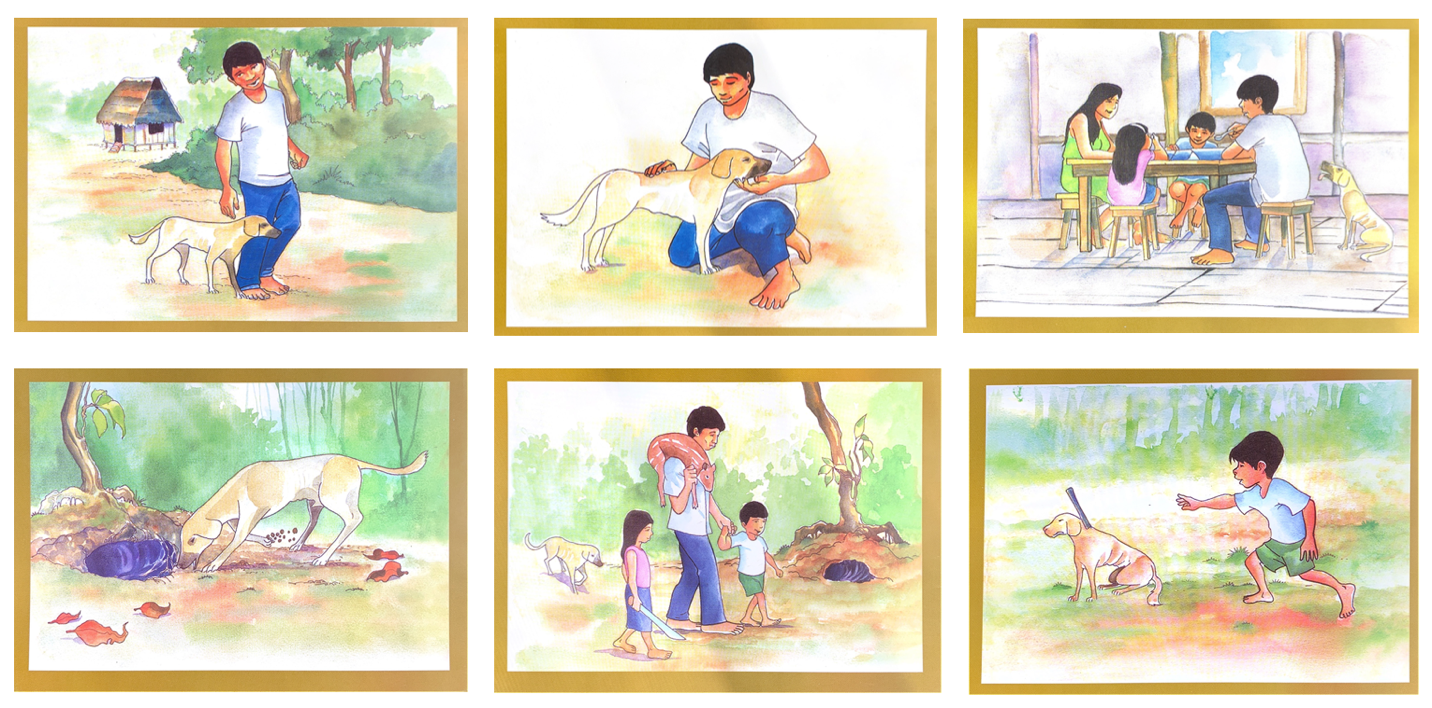
\includegraphics[width=.95\textwidth]{figures/rivera-img011.png}
\end{figure}


The participants organized the cards in the order of their preference and then proceeded to create a story. These stories were recorded to allow qualitative and quantitative analyses, including speech rate. These speech samples are rich in objectively recognizable linguistic features in the areas of phonetics, phonology, morphology, syntax, discourse, and lexicon. It is important to note, however, that this procedure elicits samples of what speakers can do and help us identify areas of improvement, but it is not necessarily useful for discovering areas that speakers do not know yet. In the future, we may need to include other tasks to capture what advanced learners cannot do and need focused help with.

\subsection{{{Questionnaire}}}

We created a questionnaire to collect biographical information to determine what social and cultural factors influence their attitudes, motivations, and linguistic choices (cf. \citealt{Alarcon2010}).~It includes 32 items in total. The political and affective issues surrounding heritage speakers came to light in these questionnaires. The first portion elicits information regarding their exposure to their ancestral languages during childhood, their motivations to become bilingual teachers, and their knowledge of their ancestral language before coming to FORMABIAP. In the second part of the questionnaire we collected information regarding language behaviors, attitudes towards dialectal and generational variation, and self-assessments of their heritage language abilities. Data from the questionnaire allows the examination of potential correlations between self-reported proficiency level, and speech rate, word recognition, and the use of specific grammatical patterns.

In the next section, we present preliminary findings on linguistic correlates of proficiency in Kukama and Kichwa as heritage languages, based on data from the questionnaires, as well as perception and production tasks.

\section{{Results: Kukama}}\label{sec:7:5}

This study looks at five Kukamas. They are all heritage speakers that entered the program with very limited knowledge of their ancestral languages. The profiles of the participants in which group is described in detail below.

\subsection{{{Participant profiles}}}

\begin{sloppypar}
Five heritage speakers of Kukama, four males and one female, participated in this study. Their ages ranged from 24 to 36 (avg = 28), and they all attended FORMABIAP between 2012 and 2016.\footnote{{The participants attended a propaedeutic in 2011, before starting their teaching training, but Kukama was not included in this preparatory phase.}} They had two male instructors of Kukama, who are themselves community members and FORMABIAP alumni (see \sectref{sec:7:3.2}). During their training, they were also mentored by four Kukama specialists, two male and two female elder speakers, who worked in the project at different points in time.
\end{sloppypar}

Data from anonymous questionnaires show that after finishing high school, they all wanted to become bilingual teachers, and four of the five participants indicated having the support from their communities and indigenous organization. As for their exposure to Kukama at an early age, four of the five participants indicated that their parents understand the language and that their grandparents would speak it, but only from time to time because they lack regular conversation partners. All the participants are aware of the level of endangerment of Kukama and seem committed to ongoing preservation efforts. They display very positive attitudes towards their Kukama identity and their heritage language; however, four of the five participants indicated they prefer not to speak Kukama outside their community contexts to avoid public shame. As for language ideologies regarding language variation, all the participants acknowledge geographic and generational differences; however, four of the five participants indicated they aspire to speak like the elders because they speak the true Kukama.

\begin{sloppypar}
Regarding their knowledge of Kukama at the time they enrolled in FORMABIAP, all of the participants say they knew common words and expressions. For words, the examples provided in the questionnaire are \textit{ipira} ‘fish’, \textit{yawara} ‘dog’ \textit{atawari} ‘chicken’, \textit{arara} ‘macaw’, \textit{uni} ‘water’, \textit{irara} ‘canoe’, ‘\textit{yapukita} ‘paddle’, etc. For expressions, they listed: \textit{era na kuema/karuka} ‘good morning/afternoon,’ \textit{tsaniuri} ‘Come on in’, \textit{makatipa na utsu} ‘Where are you going’, \textit{ta tseta eyu} ‘I want to eat’, \textit{ta kurata kaitsuma} ‘I drink yucca bear’. Even though they knew some words and expressions, all of them said they could not understand and engage with fluent speakers of Kukama. In the self-assessment of their proficiency, all declared having made significant progress in learning the language. On a 5-point scale, they gave themselves an average score of 4.2 for reading and writing, and 3.2 for speaking and listening.
\end{sloppypar}

Given the lack of baselines and benchmarks to assess proficiency in Kukama, a fluent, elder speaker with 20 years of experience as the community linguist, and who was an instructor of the Kukama language in the FORMABIAP project, assessed the speech samples of all the participants. She listened to each story and grouped the participants into three categories: A: \textit{está aprendiendo} `he/she is learning', B: \textit{habla, pero tiene que aprender y practicar más} `he/she speaks, but needs to learn and practice more', C: \textit{ya habla, pero necesita corregir algunas palabritas} `he/she speaks already, but needs to fix some little expressions'. We interpret these categories as A being towards the lower end of the proficiency continuum, and C towards the higher end of the continuum. According to this specialist, the participant \textsc{kuk}{}-1 should be in category A, \textsc{kuk}{}-2 and \textsc{kuk}{}-3 in category B, and \textsc{kuk}{}-4 and \textsc{kuk}{}-5 in category C. The profiles of the Kukama participants is summarized in \tabref{tab:7:2}.

\begin{table}
\caption{Kukama participants}
\label{tab:7:2}
\begin{tabularx}{\textwidth}{QXXl}
\lsptoprule
Participant & Gender & Age & Category\\
\midrule
\textsc{kuk}{}-1 & M & 36 & A\\
\textsc{kuk}{}-2 & M & 28 & B\\
\textsc{kuk}{}-3 & F & 24 & B\\
\textsc{kuk}{}-4 & M & 27 & C\\
\textsc{kuk}{}-5 & M & 25 & C\\
\lspbottomrule
\end{tabularx}
\end{table}

\subsection{{{Oral comprehension}}}

The data to assess oral comprehension comes from the activities with the video as explained in \sectref{sec:7:4.1}. All the participants completed the word recognition task with extreme ease. Remarkably, four of the five participants listed only those items that they clearly knew; only one participant listed a couple of nonwords, which were excluded from the counting. The vast majority of the items registered were content words, including nouns (e.g. \textit{marawi} ‘hand fan’, \textit{mɨrɨti} ʼpalm treeʼ), verbs (e.g. \textit{imaki} ‘selectʼ, \textit{kauki} ‘waitʼ ), and adverbs (e.g. \textit{ikun} ‘today’, \textit{ikumenan} ‘soon’); only one participant listed also a few function words, such as pronouns and demonstratives (ex. \textit{ay} ‘he/she’, \textit{ajan} ‘this’). We included both of them in our calculations.

The second task consisted of identifying phrases and sentences. All the participants were able to recognize and isolate a variety of syntactic structures. Within the \textsc{phrases} category we report only those that were listed on their own, not as part of another larger syntactic constituent (i.e. NP objects within a clause were not counted as phrases). This category comprises noun phrases (ex. \textit{ini puwa ‘}our hand’), verb phrases (ex. \textit{uchima tsa} ‘extract the leaf’) and nominalized constructions (ex. \textit{kuarachi tatatan} ‘something that has dried with sunlight’). Interestingly, no one listed postpositional phrases on their own. In the \textsc{clauses} category, we included simple clauses (ex. \textit{ikun kuashi ini yauki} \textit{marawi} ‘today we will make a hand fan’), complex constructions (ex. \textit{awanu tseta purepeta ajan} ‘people want to buy this’, \textit{ini yaukiai imaki ipukun} ‘we make it by selecting the long ones’). The results are provided in \figref{fig:7:2}. Note that only one participant, \textsc{kuk}{}-1, listed more phrases (n = 9) than clauses (n = 5). All the other participants registered more complete clauses than phrases, which may point towards more advanced comprehension skills. However, there are not significant differences among the participants in the overall comprehension of phrases and clauses.\footnote{$\chi^2$: 6.549, $p$: 0.161727. The result for \textit{phrases} and \textit{clauses} is not significant at $p< 0.05$. It becomes significant if we include \textit{words}.} In sum, the data suggests that all the participants have achieved strong comprehension skills.

\begin{figure}
\caption{Kukamas’ oral comprehension}
\label{fig:7:2}
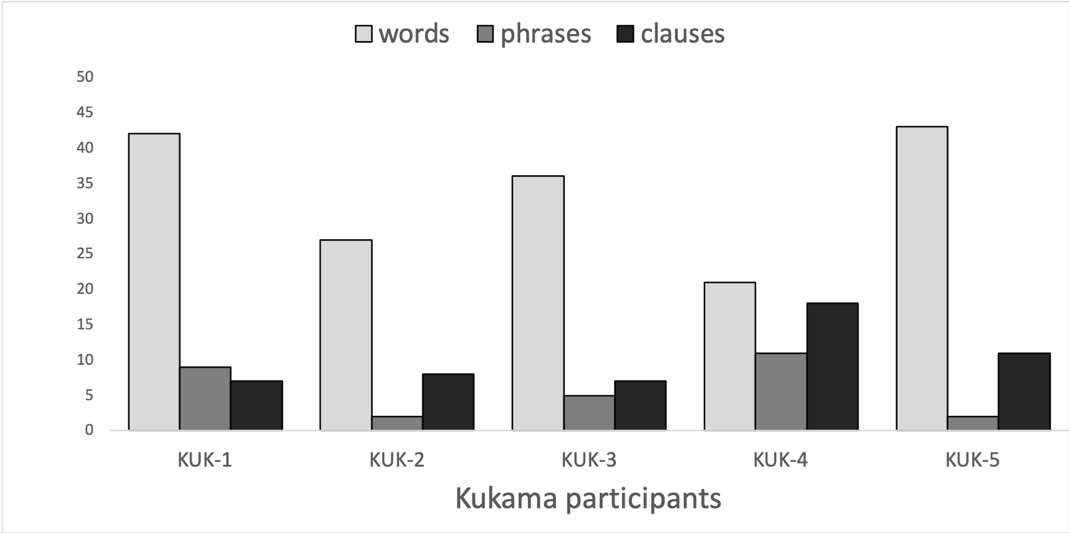
\includegraphics[width=\textwidth]{figures/rivera-img012.png}
\end{figure}

\subsection{{{Oral production}}}

As with the comprehension tasks, we let the benchmarks for Kukama oral proficiency emerge from the data itself. The literature on heritage language teaching and learning suggests that heritage learners follow unique trajectories and should not be compared against traditional speakers (see, for instance, \citealt{Valdés2005}). Following this view, the benchmark to measure oral proficiency in this study is not the speech of the elders. In collaboration with speakers of the language, we transcribed the recordings of the stories produced by the participants to quantify several parameters. First, because each participant was invited to speak for as long as he/she wanted, we recorded the length of each story. Second, we quantified the total number of words used. Third, we calculated the number of word types (including both function words and content words) to get a sense of vocabulary knowledge and the amount of repetition of words. Finally, we calculated speaker rates as word-per-minute output by dividing the total number of words by the length of the stories. The idea being that lower proficiency speakers have more difficulty in accessing lexical items, which slows down their speech. The results for both stories are provided in \figref{fig:7:3}.

The results for oral production suggest that participant \textsc{kuk}{}-1 is at a lower level in the proficiency continuum compared to the other participants, particularly with respect to the length of the stories and the overall number of words produced. \textsc{Kuk}{}-1’s score for word types (n = 55) is also lower than the average for all the participants (avg = 94). However, a chi-square test comparing word types and speech rate reveals that there is not a significant difference among the participants.\footnote{$\chi^2$: 4.4693, $p$: 0.346208. The result for \textit{word types} and \textit{speech rate} is not significant at $p < 0.05$. It becomes significant if we add \textit{number of words}.}

\begin{figure}
\caption{Kukamas’ word tokens and types in oral production}
\label{fig:7:3}
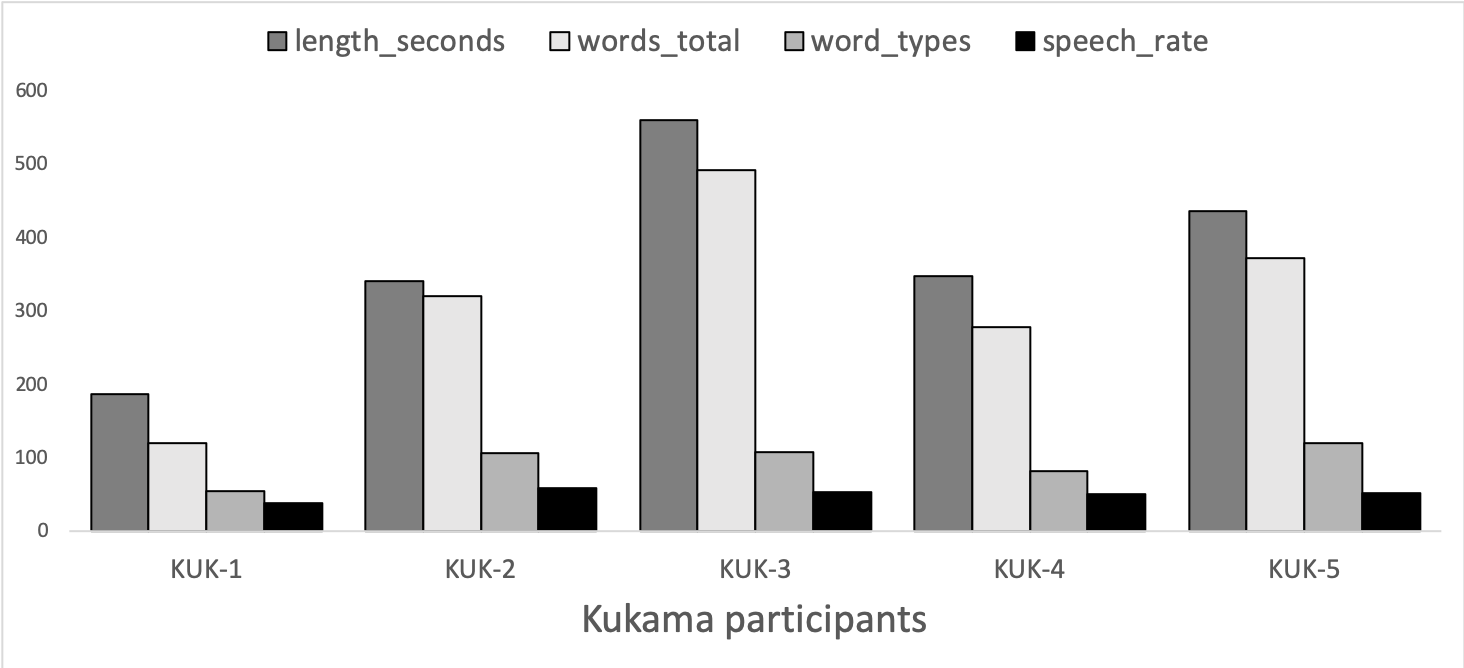
\includegraphics[width=\textwidth]{figures/rivera-img013.png}
\end{figure}


An interesting finding is that the assessment provided by the Kukama specialist does not align well with some scores in \figref{fig:7:3}. While her observations regarding \textsc{kuk}{}-1 seem to hold, according to this specialist, participant \textsc{kuk}{}-3 should be a little behind participants \textsc{kuk}\nobreakdash-4 and \textsc{kuk}\nobreakdash-5. Nevertheless, as shown in \figref{fig:7:3}, \textsc{kuk}{}-3 has the highest scores for total number of words produced and word types employed. Thus, these scores offer only a glimpse into the story of this relearning process. In order to have a fuller picture, and guided by the specialist’s observations, we look into specific linguistic features produced by the participants.


\subsection{Qualitative analysis}

Our results suggest that knowledge of lexical items and speech rate might not be correlated with grammatical knowledge and pragmatic competence. This seems surprising given that lexical access tends to also be accompanied by difficulty constructing phrases and clauses. Thus, some discussion of the results on specific subcomponents of the grammar are in order.

\subsubsection{­Phonetics and phonology}
A recurrent observation about heritage speakers is that even the novice sound native-like, which contrasts with what we see in conventional second languages \citep{PolinskyKagan2007}. This holds true for the Kukamas as well. For instance, impressionistically, their intonation patterns sound comparable to fluent speakers. Stress assignment is always on target; it is realized in the penultimate syllable except in words that end in a consonant (ex. \textit{éyu} ‘eat’, \textit{eyún} ‘food’). Phonological processes are consistently implemented (ex. sonorization of voiceless stops following nasals, as in \textit{temente} [temende] ‘there is not’, \textit{ajanka} [ajanga] ‘here’).
Optional phonological processes are implemented randomly (palatalization of affricate \textit{tsitsa} [chitsa{]} `face'). All participants tend to produce the central vowel /ɨ/, as /i/. Arguably, they have not added yet this vowel to their vowel inventory.

\subsubsection{Morphosyntax}
In Kukama, grammatical categories such as person, number, tense, and modality are conveyed by positionally fixed clitics. All the participants make use of a subset of these forms. Importantly, given that no suffix or clitic is obligatory in Kukama, the lack of bound morphology do not render structures ungrammatical. The most frequently used postpositions are -{\textit{ka}}{ ‘locative’, -}{\textit{pu}}{ ‘instrument’, -}{\textit{muki}}{ ‘comitative’, and -}{\textit{kuara}}{ ‘inesive’. Documented verbal morphology include -}{\textit{ka}}{ ‘iterative’, -}{\textit{ta}}{ ‘causative’, -}{\textit{ari}}{ ‘progressive’. The completive -}{\textit{pa}}{ was not documented, and the use of past tense markers is also limited. All the participants also used plural markers and nominalized forms and their underived counterparts. Some examples are} {\textit{eyu}}{ ‘eat’,} {\textit{eyun}}{ ‘food’} {\textit{ipurkari}}{ ‘hunt’,} {\textit{ipurkarin}}{ ‘hunter’. The focus clitic =}{\textit{pura}} was used by two participants, and generally with the same host which suggests they learned it is a chunk, as shown in \xref{ex:7:1}.

\ea\label{ex:7:1}
\gll  rian=\textit{pura} ikian     awa=\textit{kana} umi ra yawara\\
  then=\textsc{foc}  \textsc{dem.ms}  person-\textsc{pl.ms}  see  \textsc{3sg.ms}   dog\\
\glt ‘at that moment these people see his dog’
\z

One of the most salient typological features of Kukama is the presence of grammaticalized gender indexicals (for details, see \citealt{Vallejos2015}). Kukama does not have grammatical gender; that is, it does not encode the gender of a referent. Kukama’s gender indexicality is a categorical distinction that encodes the gender of the speaker. Male and female speech is expressed in several categories, including personal pronouns, indefinite pronouns, demonstratives, number marking, and connectors. Heritage speakers use plural markers, as =\textit{kana} in \xref{ex:7:1}, and the first-person pronouns (\textit{ta} vs\textit{. tsa/etse}) quite accurately. The second-person pronoun, \textit{na}, does not vary from women and men. However, some of the participants tend to have difficulties with third-person pronouns (\textit{uri/ra} vs. \textit{ya/ai}) and, the first-person exclusive pronouns (\textit{tana} vs\textit{. penu}) did not show up in the stories. Although one male participant used a few female forms (\textit{yamua} instead of \textit{ramua} ‘other’, \textit{yaepetsui} instead of \textit{raepetsui} ‘then’), male speakers consistently used male pronouns, as \textit{ra} in \xref{ex:7:1}. The female speaker had more difficulties with gender indexicals, as discussed further, below.

Kukama has several strategies to combine clauses into more complex sentences. Clause nominalization is a central subordination strategy, particularly for relativization functions. The language has a set of subordinators to express several logical relations, such as cause, condition, and temporal simultaneity \citep{Vallejos2016a}. The participants made very limited use of clause combining strategies.\footnote{ {Two of the five participants used two purpose subordinators at once, but with the same verb (}{\textit{eyu-mira-tsen}} {eat-\textsc{pur}2-\textsc{pur}3). This sequence may have been learned as a single chunk.}} To link simple clauses, they use prosody; clauses are produced within a single intonation contour and the semantic relationship between clauses are left to be inferred from context, as shown in \xref{ex:7:3}. This is an area that needs attention.

An area that seems to represent a challenge is information questions. Kukama has the interrogative marker -\textit{tipa} that is attached to an interrogative pronoun, or the piece of information under interrogation. Only two participants attempted to make questions with this morpheme, the others used only rising intonation. However, the syntactic structure of the attempted questions tends to be problematic, as shown in example \xref{ex:7:2a}, produced by \textsc{kuk}\nobreakdash-5. In \xref{ex:7:2a}, the sentence has an interrogative pronoun, but the interrogative marker is in the verb. Also, the subject of the clause is missing. The Kukama specialist provided two potential target constructions according to the context of the story, which are given in \xref{ex:7:2b}. %(2$\prime$).
In the first, the identity of the object is being interrogated. In the second, the predicate is being interrogated, but in this case the object argument needs to be realized.

\ea
  \ea\label{ex:7:2a}
  \gll  mari   tseta=\textit{tipa} eyu\\
  What  want=\textsc{int}  eat\\
  \glt ‘What want eat’ (Lit.)
  \ex\label{ex:7:2b}
  \gll mari=\textit{tipa} na   tseta   eyu   /   Tseta=\textit{tipa} eyu-n\\
  What=\textsc{int}  \textsc{2sg}  want   eat {}   want=\textsc{int}  eat-\textsc{nzr}\\
  \glt ‘What do you want to eat?’      ‘Do you want food?’
  \z
\z

It should be highlighted that some types of complex predicate constructions -- i.e., clause constructions with more than one predicate -- are employed by all of them. Some examples are provided in \xref{ex:7:3c} and \xref{ex:7:3e}, below.


\subsubsection{Discourse pragmatics}
Recall that according to the scores in \figref{fig:7:2}, the participants could be located at relatively similar points in the proficiency scale, except {\textsc{kuk}}{{}-1. However, the Kukama expert put them in three groups.} {\textsc{kuk}}{{}-2 and} {\textsc{kuk}}{{}-3 were categorized in group B (“he/she speaks but needs to learn more and practice more”), while and} {\textsc{kuk}}{{}-4 and} {\textsc{kuk}}{{}-5 in group C (“he/she speaks already, but needs to fix some expressions”) by the Kukama expert. The explanation seems to lie in the fact that their speech differs in terms of discourse organization.}

\begin{sloppypar}
Story telling is an important cultural practice among Amazonian peoples. Kukama elders are generally exceptional storytellers, and most traditional stories have a message regarding social norms and expectations in the community. These stories are told for the most part in the third person, and most of them concern animals interacting with each other and their surroundings (see an example in \citealt{Vallejos2018}). Their stories are full of dialogue and direct quotations. To incorporate direct speech from participants assigned to different sex categories, they re-center the referents of the gender indexicals for each speech event. The stories collected with the picture cards lack these features, which is perhaps explained by the artificiality of the stimuli.
\end{sloppypar}

Consider \xref{ex:7:3}, an extract from one of the stories produced by participant \textsc{kuk}{}-4. This story flows well. There is almost null use of bound morphology, but this speaker employs complex predicate constructions, as in \xref{ex:7:3a}, \xref{ex:7:3c}, and \xref{ex:7:3e}, as well as reduplication of verbal roots, as in \xref{ex:7:3e}, to express aspectual subtleties.


\ea\label{ex:7:3}
\ea\label{ex:7:3a}
\gll ra     utsu   umi   wepe,   wepe   uka   animaru\\
      \textsc{3sg.ms}  go  see  one  one   house  animal\\

\ex\label{ex:7:3b}
\gll ra     chiwiki\\
    \textsc{3sg.ms}  dig\\

\ex\label{ex:7:3c}
\gll ra     utsu   tsetuni,\\
    \textsc{3sg.ms}  go  smell\\

\ex\label{ex:7:3d}
\gll tsetuni   ria   animaru,   hm\\
    smell  too  animal    hm\\

\ex\label{ex:7:3e}
\gll ra     yupuni kari-kari\\
    \textsc{3sg.ms}  start   scrape-scrape\\
\glt ‘(a) It [hunting dog] goes to see one, a house of an animal, (b) he digs, (c) he goes to smell it, (d) to smell this animal’s (house), (e) he starts to scrape and scrape’ (\textsc{kuk}{}-4)
\z
\z

An interesting point that emerged in the speech of participants \textsc{kuk-2} and \textsc{kuk-3} is the overuse of the second person singular pronoun \textit{na} for impersonal functions. Elder, traditional speakers of Kukama do not use \textit{na} for generic, impersonal reference. In the excerpt in \xref{ex:7:4}, the speaker \textsc{kuk}{}-2 seems to be describing the activity of hunting, not creating a story about the dog. If we substitute the pronoun \textit{na} ‘you’ for \textit{ra} ‘he/she’, we would have a third person story, similar to what we see in \xref{ex:7:3}. In the extract in \xref{ex:7:5}, the participant \textsc{kuk}{}-3 uses of \textit{na} in similar ways, although in some cases, the resulting constructions are problematic and difficult to understand, as in \xref{ex:7:5d}.


\ea\label{ex:7:4}
\ea\label{ex:7:4a}
\gll na     papa,   na\\
     \textsc{2sg}    father \textsc{2sg}\\
\ex\label{ex:7:4b}
\gll na     erutsu   yawara=muki\\
   \textsc{2sg}    bring  dog=\textsc{com}\\

\ex\label{ex:7:4c}
\gll na     chikari   wepe   animaru\\
    \textsc{2sg}    look.for  one  animal\\

\ex\label{ex:7:4d}
\gll ikian,   na   papa,     na\\
    this    \textsc{2sg}  father     \textsc{2sg}\\
\ex\label{ex:7:4e}
\gll na   utsu   taira=kana\\
   \textsc{2sg}  go  daughter-\textsc{pl.ms}\\
\glt ‘(a) Your father, (b) brings you with the dog, (c) you look for an animal, (d) this one, your father, (e) you go with the daughters’
\z
\z


\ea\label{ex:7:5}
\ea\label{ex:7:5a}
\gll ajan     wepe   yawara   ipurkari-n   umi=ura\\
      this.\textsc{fs}  one  dog    hunt-\textsc{nzr}  see=\textsc{3sg.ms}\\

\ex\label{ex:7:5b}
\gll umi=ura     na   tseta   upi=nan [\ldots]\\
     see=\textsc{3sg.ms}    \textsc{2sg}  want  all=\textsc{foc}\\

\ex\label{ex:7:5c}
\gll tima     na,   na   yumi   eyu-n [\ldots]\\
   \textsc{neg}    \textsc{2sg}  \textsc{2sg}  give  eat-\textsc{nzr}\\

\ex\label{ex:7:5d}
\gll upi=nan   tua-n=kana     titi-ka     na   eyu-mira\\
   all=\textsc{foc}  big-\textsc{nzr=pl.ms}  alone-\textsc{rei}  \textsc{2sg}  eat-\textsc{pur}\\

\ex\label{ex:7:5e}
\gll tima     na   yumi   animaru   ipurkari-n\\
    \textsc{neg}    \textsc{2sg}  give  animal    hunt-\textsc{nzr}\\
\glt ‘(a) This hunting dog sees it [the food], (b) sees it (but) you want all, (c) you don’t share the food, (d) all the adults are alone for you to eat, (e) you don’t give to the hunting dog’
\z
\z

But why would these two participants use \textit{na} instead of \textit{ra} in story telling? One hypothesis is because the second person pronoun does not vary depending on the speaker’s gender, as does the third person (\textit{ra} vs. \textit{ya}). A second hypothesis is Spanish influence. This impersonal use of \textit{na} resembles the use of Spanish \textit{tú} for similar discourse functions in Amazonian Spanish \citep{VallejosEtAl2020}, as well as in English as evidenced in the translations.

The fragment in \xref{ex:7:5} is also interesting for other reasons. Speaker \textsc{kuk}{}-3 uses more bound morphology than other participants (i.e., the plural marker, clitic pronouns, nominalizer, focus, the subordinator of purpose), but recall that this speech was nonetheless rated lower than of \textsc{kuk}{}-4 and \textsc{kuk}{}-5. In addition to the overuse of \textit{na}, this speaker mixes gender indexicals. For instance, in \xref{ex:7:5a}, \textsc{kuk}{}-3 uses \textit{ajan}, the demonstrative of female speech, but in the same line she uses =\textit{ura}, the clitic pronoun for male speech (instead of =\textit{ay}), and in \xref{ex:7:5d} the plural marker for male speech =\textit{kana} (instead of =\textit{minu}). Traditional speakers tend to be sensitive to the use of gender indexicals. But mastering this feature is difficult, and more so if there is not enough input of both types of speech and opportunity for practice. Note that the instructors of Kukama are males. Hiring female instructors should be considered in instructional planning in the future.

An additional point to note regarding the speech of heritage speakers is the innovative uses of \textit{wepe} ‘one’. This cardinal number is used as indefinite determiner, as seen in \xref{ex:7:3a}, \xref{ex:7:4c}, and \xref{ex:7:5a}, probably because of Spanish influence. For example, everyone said \textit{wepe kuashi} ‘one day’, which would work well if we were counting days, but not to make reference to a point in time in the past. For these function, traditional speakers would use expressions such \textit{ɨmɨnua} ‘long time ago’\textit{, yamua/ramua kuashi} ‘another day’\textit{, ikun kuashi} ‘today’, etc.

A final point regarding discourse is the very limited use of code switching by these participants. They all inserted very few loanwords, but nothing that would be considered switches to Spanish. This is surprising since in a previous study, with a different speaker sample \citep{Vallejos2016b}, switching was extensively used by heritage speakers. A possible explanation is that the participants in this study have studied under different instructors.

\section{{Results: Kichwa} }\label{sec:7:6}
\subsection{{{Participant profiles}}}

Three heritage learners of Kichwa participated in this study: two women and one man. \textsc{kich}{}-1 and \textsc{kich}{}-2 are women, and their ages are 30 and 35, respectively. They attended FORMABIAP between 2015 and 2019 to get training as teachers of preschool education (\textit{Educación Inicial Intercultural Bilingüe}) during the summer periods. It needs to be highlighted that the training of preschool teachers is different from the training of elementary school teachers. The former are teachers that must have a teaching position in a preschool to attend formal training in FORMABIAP; the latter do not hold a teaching position prior to graduation. As a result, participants \textsc{kich}{}-1 and \textsc{kich}{}-2 have had limited access to structured classes of Kichwa during their time at FORMABIAP; that is, they are mostly learning the language in their villages while working with kindergarteners. The third participant is a 22-year-old man; he attended FORMABIAP from 2012 to 2017 to become an elementary school teacher. As such, he has taken classes of Kichwa during his five years at FORMABIAP.

\begin{sloppypar}
In the anonymous survey applied, two participants said they entered FORMABIAP because of the scholarship offered to carry out their studies, and because of the support of their communities and families. However, the three of them indicated that their motivation to learn Kichwa emerged in the framework of their professional training in FORMABIAP. \textsc{kich}{}-3 self-reported that, in addition to the classes at FORMABIAP, he systematically immersed himself with fluent speakers in the villages where Kichwa is the dominant language to gain proficiency.
\end{sloppypar}

\begin{sloppypar}
Regarding prior knowledge of Kichwa before entering FORMABIAP, they stated that they knew common words like \textit{challwa} `fish', \textit{wallpa} `hen', \textit{yachachikama} `teacher' and phrases like \textit{allipuncha} `good morning', \textit{shamuy} `come', \textit{kuyntaway} `tell me'. However, they may have comprehended more words and phrases because two of them said they listened to their grandparents speak Kichwa during their childhood. All three said that in their community there were older adults who spoke Kichwa fluently. That is, the three participants of this study were exposed to Kichwa during their childhood by their grandparents and other elders; however, they did not foster the use of the language because the social conditions did not exist.
\end{sloppypar}

In the same survey, the three participants indicated they are proud of the Kichwa language and think that the elders speak the true Kichwa and that the young people should learn from them. In summary, the three participants have a strong appreciation of Kichwa, which is a good motivation to continue to learn this language.

A Kichwa specialist assessed all the speech samples to provide some input regarding the overall proficiency of the participants. According to this specialist, \textsc{kich}{}-1 and \textsc{kich}{}-2 should be assigned to category B (\textit{habla, pero tiene que aprender y practicar más} `he/she speaks, but needs to learn and practice more'), while \textsc{kich}{}-3 is in category C (\textit{ya habla, pero necesita corregir algunas palabritas para hablar fluido} `he/she speaks already, but needs to fix some little expressions to speak fluently'). That is, \textsc{kich}{}-3 is the most advanced of the three in terms of proficiency. A summary of the profiles of the Kichwa participants is given in \tabref{tab:7:3}.

\begin{table}
\caption{Kichwa participants}
  \label{tab:7:3}
\begin{tabularx}{\textwidth}{QXXl}
\lsptoprule
Participant & Gender & Age & Category\\
\midrule
\textsc{kich-}1 & F & 30 & B\\
\textsc{kich-}2 & F & 35 & B\\
\textsc{kich-}3 & M & 22 & C\\
\lspbottomrule
\end{tabularx}
\end{table}

\subsection{{Oral comprehension}}

Given some technical difficulties, we could not collect oral comprehension data similar to the Kukamas. However, two Kichwa instructors who taught the three participants indicate that all of them display advanced oral comprehension to fully understand narratives and descriptions. For example, in FORMABIAP there are certain sessions conducted entirely in the Kichwa language. Those sessions are dedicated to teach both the language itself, as well as socio-cultural studies. According to the instructors, the three Kichwa participants successfully participated in those sessions, working in close collaboration with other fluent Kichwa speakers. The second and third authors have worked with these participants, and believe the three of them have achieved advanced oral comprehension skills because they are originally from the Mid Napo River. As indicated in \sectref{sec:7:2.2}, in those villages, the generations of parents and grandparents still speak the language on a daily basis; thus, the conditions to relearn Kichwa are relatively favorable.

\subsection{{{Oral production}}}

To collect oral production data, we employed a similar strategy to the one used with the Kukamas. The participants organized the sets of cards and briefly described them creating a story.

The results for the oral production task are given in \figref{fig:7:4}. They show that participant \textsc{kich}{}-3 is at a more advanced level in the proficiency continuum compared to the other two participants, particularly with respect to the length of the stories and the overall number of words produced. \textsc{kich}{}-3’s score for word types ($n = 144$) is above the average for the three participants (avg~=~92). The only score in in which \textsc{kich}{}-1 and \textsc{kich}{}-2 are above \textsc{kich}{}-3 is speech rate. However, a chi-square test comparing word types and speech rate reveals that there is not a significant difference among the participants.\footnote{$\chi^2$: 4.4693, $p$: 0.346208. The result for \textit{word types} and \textit{speech rate} is not significant at $p<0.05$. It becomes significant if we add \textit{number of words}.} The assessment provided by the Kichwa specialist aligns well with most of the scores in \figref{fig:7:4}. An analysis of specific linguistic features produced by the participants is found in \figref{fig:7:4}.

\begin{figure}
\caption{Kichwas' oral production}
\label{fig:7:4}
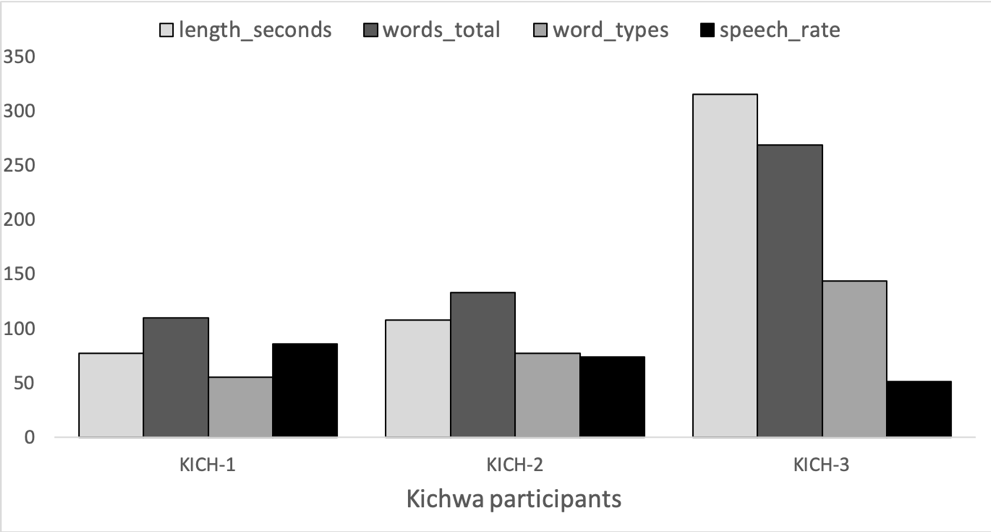
\includegraphics[width=\textwidth]{figures/rivera-img014.png}
\end{figure}

\subsection{{{Qualitative analysis}}}
\subsubsection{Phonetics and phonology}
\begin{sloppypar}
The participants \textsc{kich}-1, \textsc{kich}-2 and \textsc{kich}-3 do not differ much from fluent Kichwa speakers with respect to the production of different sounds, intonation and even accent patterns. One of the phonetic characteristics of Kichwa is the sonorization of the voiceless stops /p, t, k/ which become [b, d, g], respectively, after a nasal consonant. For example, /ñampi/ `path' is realized as [ñambi{]}, /inti/ ‘sun’ is produced as [indi{]}; /chunka/ ‘ten’ is produced as [chunga{]}. All the participants apply this voicing process. The stress pattern in Kichwa falls on the penultimate syllable, but in the spontaneous speech of fluent speakers, a word can undergo reduction of the stressed vowel, in which case the accent falls on the last syllable. For example, /manáchu/ ‘is not true’ becomes [manchú{]}. This vowel reduction phenomenon is documented in the speech of these heritage speakers as well. A related phenomenon is the fact participant kich\nobreakdash-3 stresses the last syllable of some words like [tupán{]} that are generally produced as /túpan/ `to meet someone', although this issue seems marginal.
\end{sloppypar}

\subsubsection{Morphosyntax}
Kichwa is an agglutinating, suffixal language; nominal and verbal words are constituted of a verbal and nominal root and their respective suffixes. Grammatical relations are expressed via case marking including the accusative \textit{-ta}, and the indirect object \textit{-ta} or \textit{-ma}. Non-core arguments are marked by a set of postpositions, the most frequent being the locative \textit{-pi}, the allative \textit{-ma} (when the noun is non-human), the allative \textit{\nobreakdash-pam} (when the noun is human), the ablative \textit{-manta}, and the comitative/instrumental \textit{-wa}. The main predicate of the clause is marked mainly with person indexes including: \textit{-sha} `1{\textsc{sg.fut}',} \textit{-nki }{`\textsc{2sg',}}\textit{ -nka} ‘3{\textsc{sg.fut’}}{. The main verb can also take the tense marker \textit{\nobreakdash-rka} ‘past’, aspectual markers such as \textit{-ra/-hu} ‘durative’, \textit{-shka/-ska} `perfective', and the causative marker \textit{\nobreakdash-chi}. All these morphemes are basic and frequent in everyday conversation. The preferred order of constituents in the clause is SOV, but this pattern is flexible because the core and non-core arguments are morphologically marked, with the exception of the subject argument. Thus, moving arguments around the clause does not alter the propositional meaning of the utterance, although it may change its pragmatics (\citealt{PapaCoquincheRosalesAlvarado2015}).}

The three Kichwa participants seem to know most of the morphemes listed above. Participants \textsc{kich-}1 and \textsc{kich-}2, however, are in the process of strengthening the proper use of these suffixes. Note that the presence or absence of these morphemes can change the meaning of an expression in substantial ways. The example in \xref{ex:7:6a} was extracted from the story produced by \textsc{kich-}1. It shows that this participant is learning to use the accusative -\textit{ta}, the causative -\textit{chi}, and the locative -\textit{pi.} In the context of the story, \xref{ex:7:6a} is trying to make reference to the fact that the owner of the dog makes his pet happy. This is also inferred from the transitivizer -\textit{ya} in the verb. But this example lacks the accusative marker -\textit{ta} in \textit{dog}, and the causative –\textit{chi} in the verb. The target construction provided by the Kichwa specialist is given in \xref{ex:7:6b}:%(6’):


\ea
\ea\label{ex:7:6a}
\gll   Pay-pa             allku       sumak-ta            kushi-ya-shka\\
             \textsc{3sg.pre-gen}    dog            beautiful-\textsc{advzr}     be.happy-\textsc{trs}{}-\textsc{pfv}\\
  \glt ‘His dog got happy beautifully’ (Lit)
\ex\label{ex:7:6b}
\gll Pay-pa        allku-\textit{ta} sumak-ta       kushi-ya-\textit{chi}{{}-shka}\\
\textsc{3sg.pre-gen}   dog-\textsc{acc}        beautiful-\textsc{advzr}     be.happy-\textsc{trs}{}-\textsc{cau}{}-\textsc{pfv}\\
  \glt ‘He made his dog very happy’
\z
\z

The following example was also produced by \textsc{kich-}1. It shows that the verb has the necessary morphology of a finite verb. However, this participant used the instrumental marker \-\-\nobreakdash-\textit{wa} instead of the locative marker \-\nobreakdash-\textit{pi} to indicate that the bench is where the sitting takes place. The target construction is given in \xref{ex:7:7b}.%(7’).

\ea
\ea\label{ex:7:7a}
\gll Chaymanda       chay   runa      shuk    banka-\textit{wa} tiya-ri-rka\\
         then      \textsc{dem}     person   one   bench-\textsc{ins}    sit-\textsc{inc}{}-\textsc{pas}\\
\glt          ‘Then that person sat with a bench’
\ex\label{ex:7:7b}
\gll Chaymanda       chay   runa      shuk   banka-\textit{pi} tiya-ri-rka\\
  then      \textsc{dem}     person   one   bench-\textsc{loc}    sit-\textsc{inc}{}-\textsc{pas}\\
  \glt ‘Then that person sat on a bench’
\z
\z

Participants \textsc{kich-}1 and \textsc{kich-}2 also show some inconsistencies with respect to preferred order of constituents. The speech sample of \textsc{kich-}3 also shows some of the same inconsistencies described above, but these are less frequent and mostly in the context of complex sentences.

One of the most salient morphological features of this language is the use of personal pronouns with the genitive marker -\textit{pa} to express possession within the noun phrase. For example, in [\textit{ñuka-pa yaya}] ‘my dad’, the first-person pronoun \textit{ñuka} is marked by the genitive marker \nobreakdash-\textit{pa}. In spontaneous speech, however, fluent speakers tend to drop the genitive marker, and possession is expressed by word order alone. As a result, fluent speakers have two variant constructions for adnominal possession: [PRO-pa N] and [PRO N]. Participants \textsc{kich-}1 and \textsc{kich-}2 are able to use the first variant, with the genitive marker. However, \textsc{kich-}3 already uses both variants, as shown in \xref{ex:7:8} and \xref{ex:7:9}. Note that, in \xref{ex:7:8}, the suffix -\textit{pa} is missing in [\textit{pay wasima}] ‘at his house’. Thus, \textsc{kich-}3 seems not only aware of the morphosyntactic variants but uses both of them effectively, which contributes to propel him towards the more advanced end of the proficiency continuum.

\begin{exe}
\ex\label{ex:7:8}
\gll    allku    pay-\textit{pa} amu-ta            riku-sa \textit{pay}{{}-}\textit{pa} chupa-ta    kuyu-ri-rka\\
          Dog  3\textsc{sg-gen}      owner-\textsc{acc}     see-\textsc{mod}  3\textsc{sg-gen}     tail-\textsc{acc}   move-\textsc{inc-pas}\\
\glt  ‘Looking at his owner, the dog moved his tail’
\end{exe}

\begin{exe}
\ex\label{ex:7:9}
\gll wayu-kuna-ta      apa-sa           ri-n \textit{pay} wasi-ma\\
           fruit-\textsc{pl-acc}       carry-\textsc{mod}    go-3\textsc{sg}   \textsc{3sg}   house-\textsc{all}\\
  \glt ‘He goes to his house carrying fruits’
\end{exe}

To form complex sentences, Kichwa employs subordinator suffixes, such as -\textit{pi} to express ‘temporal overlap’, -\textit{sha}/-\textit{sa} to express ‘manner’, and \nobreakdash-\textit{nkapa} to express the purpose of the action conveyed in the main clause. \textsc{kich}{}-3 uses all these complex structures, as shown in the following extract from a story produced by this participant. Subordinators are employed in \xref{ex:7:10b}, \xref{ex:7:10c}, and \xref{ex:7:10d}. Participants \textsc{kich}{}-1 and \textsc{kich}{}-2 use mostly sequences of simple clauses, although they tend to join them using discourse connectors, as shown in \xref{ex:7:11}, below.


\ea\label{ex:7:10}
\ea\label{ex:7:10a}
\gll  Mama     rima-n          pay-pa          wawa-kuna-ta:\\
  mother    speak-\textsc{3sg}  \textsc{3sg}{}-\textsc{gen}  son-\textsc{pl}{}-\textsc{acc}\\

\ex\label{ex:7:10b}
\gll   ``maska-kri-sha  wayu-kuna-ta    kan-kuna-ta  kara-\textit{nkapa}.''\\
  look.for-go\textsc{{}-}1\textsc{sg.fut}  fruit-\textsc{pl-acc}    2\textsc{sg-pl-ben}  give\textsc{{}-}\textsc{pur}\\

\ex\label{ex:7:10c}
\gll   chasna   rima-\textit{pi},  pay-pa    mama puri-\textit{sa} sacha-man  ri-n,\\
           like.this  speak-\textsc{temp}  \textsc{3sg-gen}  mother  go.around-\textsc{man} jungle-\textsc{all}  go-\textsc{3sg}\\

\ex\label{ex:7:10d}
\gll    sacha-pi           puri-\textit{pi} tupa-n             mishki      muyu-kuna-ta\\
jungle-\textsc{loc}  go.around-\textsc{temp}  find-\textsc{3sg}  sweet    seed-\textsc{pl}{}-\textsc{acc}\\
\glt ‘(a) Mother speaks to her sons. (b) “I’ll go look for fruits in order to give you (to feed you)”. (c) Speaking like this, mother goes walking around towards the jungle. (d) When she was walking around in the jungle, she found sweet seeds’
\z
\z

\subsubsection{Discourse pragmatics}
At the discourse level, there is a tendency to use connectors to link ideas conveyed in simple structures. This is particularly evident in the speech of {\textsc{kich}}{{}-1 and} {\textsc{kich}}{ 2. The extract below from a story by} {\textsc{kich}}{{}-1 shows this. The frequent use of} {\textit{chaymanda}}{ ‘then’ and adverbs of time such as} {\textit{washa}}{ ‘then, later’ is noticeable, as in \xref{ex:7:11a} and \xref{ex:7:11d}. This speaker seems to be using connectors instead of subordinators to link clauses.}


\ea\label{ex:7:11}
\ea\label{ex:7:11a}
\gll   Pay-pa         amu   wawa   hampi-naya-shka\\
    \textsc{3sg-gen}  owner  kid  cure-\textsc{des-pfv}\\

\ex\label{ex:7:11b}
\gll   chay   allku   mana   muna-rka\\
          \textsc{dem}  dog  \textsc{neg}  want-\textsc{pas}\\

\ex\label{ex:7:11c}
\gll   \textit{chaymanda} chay   runa   wan–chi-shka  chay   lumucha-ta\\
       then    \textsc{dem}  person  die-\textsc{cau}{}-\textsc{pfv}  \textsc{dem}  agouti-\textsc{acc}\\

\ex\label{ex:7:11d}
\gll   wan-chi-shka \textit{washa} pay-pa           wasi-ma         ri-rka\\
    die-\textsc{cau}{}-\textsc{pfv} after \textsc{3sg-gen}  house-\textsc{all}  go-\textsc{pas}\\
\glt ‘(a) His owner, the kid, wanted to cure him [the dog]. (b) that dog didn’t want to. (c) then that person killed the agouti. (d)After killing, he went to his house.’
\z
\z


An important feature of Kichwa is the focalizer -\textit{ka}. This marker operates at the level of discourse to explicitly highlight a piece of information about which one wants to draw attention. Focalization strategies are an interesting aspect in the learning process of heritage speakers. The only participant that makes use of this suffix is \textsc{kich}{}-3; however, he makes an excessive use of the focalizer, as evidenced in \xref{ex:7:12} and \xref{ex:7:13}. In sentence \xref{ex:7:12}, three elements are focalized, in \xref{ex:7:13} four elements. Fluid, native speakers focus only one element per sentence.

\begin{exe}
\ex\label{ex:7:12}
\gll    Sacha-pi         puri-pi-\textit{{ka}} allku-\textit{{ka}} ña          mushti-sa-\textit{{ka}} kati-n shuk   sacha   wiwa-ta.\\
  jungle-\textsc{loc}  go.around-\textsc{loc-}\textsc{foc}  dog-\textsc{foc}   already   smell-\textsc{man}{}-\textsc{foc}  follow-\textsc{3sg}  one  monte  animal-\textsc{acc}\\
\glt ‘When a dog goes around in the jungle, he chases a wild animal by smelling’
\end{exe}

\begin{exe}
\ex\label{ex:7:13}
\gll wan-chi-ska   washa-\textit{{ka}},   ña    all-kuna-\textit{{ka}} karachupa   wawa-kuna-ta-\textit{{ka}} wan-chi-pi-\textit{{ka}} sakinaku-n\\
  die-\textsc{cau}{}-\textsc{pfv}  after-\textsc{foc}  already   dog-\textsc{pl-}\textsc{foc}  armadillo  breed-\textsc{pl-acc-}\textsc{foc} die-\textsc{cau-temp-foc}  leave-\textsc{3sg}\\
\glt     ‘After killing the armadillo’s babies, the dogs leave them dead’
\end{exe}

Participants \textsc{kich}\nobreakdash-1 and \textsc{kich}\nobreakdash-2 do not employ the focalizer marker. In sum, some areas of pragmatics pose significant challenges for heritage learners of both Kichwa and Kukama.


\section{{Implications for instruction of heritage languages in Amazonia}}\label{sec:7:7}

The aim of this study was to explore how much heritage speakers can achieved in the process of relearning their ancestral languages in higher education programs. An examination of the use of Kukama and Kichwa as a response to audiovisual stimuli by eight FORMABIAP alumni reveals that heritage languages can be relearned in the context of formal education, as long as other forces and context dynamics are present as well. Overall, all the Kukama and \textsc{K}ichwa heritage speakers in this study demonstrated strong comprehension skills and have also achieved varying degrees of production skills. Speakers show some patterns from beginners, to intermediate levels, to quite advanced proficiency.

In addition, this study found that some features found in the speech of heritage speakers are similar to those found in the speech of elder speakers, but there are also some distinctive emerging patterns. Some of them are listed in \tabref{tab:7:4}.

\begin{table}
\caption{Some patterns identified in the speech of heritage speakers}
  \label{tab:7:4}
\begin{tabularx}{\textwidth}{QQ}
\lsptoprule
\textbf{Kukama} & \textbf{Kichwa}\\
\midrule
\multicolumn{2}{l}{\textbf{Phonetics and phonology}}\\
\tablevspace
 Participants master most sounds, stress and intonation patterns        &   Participants master most sounds, stress and intonation patterns   \\
 \tablevspace
Participants tend to produce the central vowel /\textit{ɨ}/ as [i]     &   Participants apply some general phonological rules                \\

\tablevspace
\multicolumn{2}{l}{\textbf{Morphology}} \\
 \midrule
 Participants know a subset of postpositions and clitics  &  Participants know most case and tense suffixes                        \\
\tablevspace
 Participants use few pronominal gender indexicals        &  Participants are strengthening the use and combination of suffixes    \\

\tablevspace
\multicolumn{2}{l}{\textbf{Syntax}}\\
\midrule
 Participants know basic declarative clauses and attempt interrogative constructions &    Participants know basic declarative clauses and attempt different word order possibilities    \\
\tablevspace
 Participants employ prosody to link simple clauses instead of clause subordinators  &    Some participants use clause subordinators, others use sequences of simple clauses            \\

\tablevspace
\multicolumn{2}{l}{\textbf{Discourse pragmatics}}\\
\midrule
 Participants use personal pronouns for impersonal functions in narratives     &   Participants use focalizing strategies in narratives                                              \\
\tablevspace
 Participants employ reported speech instead of direct speech                  &   Participants focalize multiple pieces of information per clause instead of selecting only one     \\
\lspbottomrule
\end{tabularx}
\end{table}

The findings in \tabref{tab:7:4} are hardly surprising, as accelerated language change is expected in contexts of language endangerment and language revitalization (\citealt{Hinton2001}, \citealt{Vallejos2016b}). For example, speakers of Navajo (Athabaskan), recognize themselves as either traditionalists and non-traditionalists. The use of Navajo specialized vocabulary, as well as some structural features such as the hierarchy of classification of nouns \citep{Hale1973}, is very rare among non-traditional speakers \citep{HolmEtAl2003}. Another example comes from Blackfoot (Algonquian). There are two varieties referred to as Old or High Blackfoot, spoken by elders, and New or Modern Blackfoot, spoken by the new generations. Among the features found in High Blackfoot is the extensive use of incorporation; however, this pattern is no longer used by the Modern Blackfoot speakers (\citealt{MiyashitaCrow2006}). In the Amazon, \citet{DanielsenTerhartInReview} report several structural innovations among latent-speakers of Baure (Arawakan). Thus, it is important to document the progress made by these learners, as well as the innovations that might be emerging in their speech.

Given that languages are surrounded by variation and diversity, we do not believe language instruction should be restricted to achieve an abstract ideal of standard. Yet the findings of this study point to some areas that may need attention in terms of curricula development. Providing specific suggestions for heritage language instruction is beyond this paper, but the analysis provided here could be taken as a starting point for Kukama and Kichwa. For example, given the central role of orality in the life and social organization of the communities, facilitating greater exposure and practice of storytelling could help the progress of heritage learners. In addition, practical activities, such as the description of specific processes and concrete objects, activities with visual stimuli such as those used here, could help promote oral production and the expansion of vocabulary. The design of grammar instruction sessions aimed at overcoming difficulties with specific patterns, for example some of those listed in \tabref{tab:7:4}, seems desirable. Finally, the need to build a community of practice cannot be underestimated. Real interaction outside the classroom with those who speak the heritage languages is key to progress in the learning process.

Another important finding of this study is the positive attitudes shown by all the participants towards their identity and their heritage languages. To relearn a heritage language, particularly one with limited communicative functionality and prestige, motivation and commitment seem crucial. In addition, documenting progress is also important. Setting achievable goals, developing autonomy, and continuous self-assessment of learning are critical.

The assessment of heritage language learners should go way beyond language skills and explicit grammatical knowledge. A holistic approach must include also pragmatic knowledge, including the control of socio-cultural language norms, as well as awareness of linguistic variation in their communities. As indicated above, language attitudes and ideologies surrounding these languages, as well as learners’ cultural connection with their ethnic group should be part of the picture as well. Finally, their political positioning with respect to their communities and indigenous organizations is also essential, especially in the context of the Peruvian Amazon.


\section{Closing remarks}\label{sec:7:8}

Language revitalization initiatives have been taking place in Latin American for some time now; however, the impact of such efforts in the creation of new speakers has not been documented thoroughly. There is a need to establish the baseline for each heritage language. This task requires detailed knowledge of each specific language, the sociocultural context, the demographic patterns of dialectal variation, etc. For Amazonian languages, this information is generally not available or systematized, and would need to be collected prior to a serious assessment of specific revitalization initiatives.

Given the degree of endangerment of the heritage languages involved, especially for Kukama and for some Kichwa villages, a significant finding of this study is that endangered languages can be relearned in well-structured instructional settings. We demonstrate that the outcomes of the methodology implemented by FORMABIAP are both tangible and substantial. The results reported here can help advance the discussion about model design and strategies to work with heritage languages within the classroom and beyond. One of the most important findings is the participants’ commitment to their language, their community, and their indigenous organizations. They express a strong motivation to continue to learn their heritage language as they teach it to children. It should be clear by now that Kukama and \textsc{K}ichwa are not conventional second languages and should not be treated as such in higher education. What pedagogical challenges heritage learners of indigenous languages bring to the classroom is an important question, and we hope to have contributed to the start of this discussion with this study.

\section*{Acknowledgments}
Our deepest gratitude goes to the eight Kukamas and Kichwas that have participated in this study. We gratefully acknowledge the contributions of Rosa Amías Murayari and Claudio Papa Coquinche, the Kukama and Kichwa specialists, respectively, who have helped us with the analysis of the data. This paper has benefited greatly from comments and discussions with Richard Ricopa Yaicate and Juan Manuel Vásquez Murayari, instructors of FORMABIAP, as well as three anonymous reviewers and the editors of the volume. Institutional support from Never Tuesta, the Coordinator of FORMABIAP, is also gratefully acknowledged. All errors and shortcomings are our own.


\section*{Abbreviations}

\begin{tabularx}{.5\textwidth}{@{}lQ}
\textsc{acc}& accusative\\
\textsc{advzr}& adverbializer\\
\textsc{cau}& causative\\
\textsc{com}& comitative\\
\textsc{dem}& demonstrative\\
\textsc{inc}& incoative\\
\textsc{int}& interrogative\\
\textsc{foc}& focus\\
\textsc{fut}& future\\
\textsc{loc}& locative\\
\end{tabularx}\begin{tabularx}{.5\textwidth}{lQ@{}}
\textsc{man}& manner\\
\textsc{ms}& male speech\\
\textsc{nzr}& nominalizer\\
\textsc{pas}& past\\
\textsc{pfv}& perfective\\
\textsc{pre}& present\\
\textsc{pur}& purpose\\
\textsc{temp}& temporal overlap\\
\textsc{trs}& transitivizer\\
 \\
\end{tabularx}

\sloppy
\printbibliography[heading=subbibliography,notkeyword=this]

\end{document}
